
%% bare_conf.tex
%% V1.4b
%% 2015/08/26
%% by Michael Shell
%% See:
%% http://www.michaelshell.org/
%% for current contact information.
%%
%% This is a skeleton file demonstrating the use of IEEEtran.cls
%% (requires IEEEtran.cls version 1.8b or later) with an IEEE
%% conference paper.
%%
%% Support sites:
%% http://www.michaelshell.org/tex/ieeetran/
%% http://www.ctan.org/pkg/ieeetran
%% and
%% http://www.ieee.org/

%%*************************************************************************
%% Legal Notice:
%% This code is offered as-is without any warranty either expressed or
%% implied; without even the implied warranty of MERCHANTABILITY or
%% FITNESS FOR A PARTICULAR PURPOSE! 
%% User assumes all risk.
%% In no event shall the IEEE or any contributor to this code be liable for
%% any damages or losses, including, but not limited to, incidental,
%% consequential, or any other damages, resulting from the use or misuse
%% of any information contained here.
%%
%% All comments are the opinions of their respective authors and are not
%% necessarily endorsed by the IEEE.
%%
%% This work is distributed under the LaTeX Project Public License (LPPL)
%% ( http://www.latex-project.org/ ) version 1.3, and may be freely used,
%% distributed and modified. A copy of the LPPL, version 1.3, is included
%% in the base LaTeX documentation of all distributions of LaTeX released
%% 2003/12/01 or later.
%% Retain all contribution notices and credits.
%% ** Modified files should be clearly indicated as such, including  **
%% ** renaming them and changing author support contact information. **
%%*************************************************************************


% *** Authors should verify (and, if needed, correct) their LaTeX system  ***
% *** with the testflow diagnostic prior to trusting their LaTeX platform ***
% *** with production work. The IEEE's font choices and paper sizes can   ***
% *** trigger bugs that do not appear when using other class files.       ***                          ***
% The testflow support page is at:
% http://www.michaelshell.org/tex/testflow/


%\documentclass[conference]{IEEEtran}
\documentclass{IEEEtran}
% Some Computer Society conferences also require the compsoc mode option,
% but others use the standard conference format.
%
% If IEEEtran.cls has not been installed into the LaTeX system files,
% manually specify the path to it like:
% \documentclass[conference]{../sty/IEEEtran}





% Some very useful LaTeX packages include:
% (uncomment the ones you want to load)


% *** MISC UTILITY PACKAGES ***
%
%\usepackage{ifpdf}
% Heiko Oberdiek's ifpdf.sty is very useful if you need conditional
% compilation based on whether the output is pdf or dvi.
% usage:
% \ifpdf
%   % pdf code
% \else
%   % dvi code
% \fi
% The latest version of ifpdf.sty can be obtained from:
% http://www.ctan.org/pkg/ifpdf
% Also, note that IEEEtran.cls V1.7 and later provides a builtin
% \ifCLASSINFOpdf conditional that works the same way.
% When switching from latex to pdflatex and vice-versa, the compiler may
% have to be run twice to clear warning/error messages.






% *** CITATION PACKAGES ***
%
%\usepackage{cite}
% cite.sty was written by Donald Arseneau
% V1.6 and later of IEEEtran pre-defines the format of the cite.sty package
% \cite{} output to follow that of the IEEE. Loading the cite package will
% result in citation numbers being automatically sorted and properly
% "compressed/ranged". e.g., [1], [9], [2], [7], [5], [6] without using
% cite.sty will become [1], [2], [5]--[7], [9] using cite.sty. cite.sty's
% \cite will automatically add leading space, if needed. Use cite.sty's
% noadjust option (cite.sty V3.8 and later) if you want to turn this off
% such as if a citation ever needs to be enclosed in parenthesis.
% cite.sty is already installed on most LaTeX systems. Be sure and use
% version 5.0 (2009-03-20) and later if using hyperref.sty.
% The latest version can be obtained at:
% http://www.ctan.org/pkg/cite
% The documentation is contained in the cite.sty file itself.






% *** GRAPHICS RELATED PACKAGES ***
%
\ifCLASSINFOpdf
  % \usepackage[pdftex]{graphicx}
  % declare the path(s) where your graphic files are
  % \graphicspath{{../pdf/}{../jpeg/}}
  % and their extensions so you won't have to specify these with
  % every instance of \includegraphics
  % \DeclareGraphicsExtensions{.pdf,.jpeg,.png}
\else
  % or other class option (dvipsone, dvipdf, if not using dvips). graphicx
  % will default to the driver specified in the system graphics.cfg if no
  % driver is specified.
  % \usepackage[dvips]{graphicx}
  % declare the path(s) where your graphic files are
  % \graphicspath{{../eps/}}
  % and their extensions so you won't have to specify these with
  % every instance of \includegraphics
  % \DeclareGraphicsExtensions{.eps}
\fi
% graphicx was written by David Carlisle and Sebastian Rahtz. It is
% required if you want graphics, photos, etc. graphicx.sty is already
% installed on most LaTeX systems. The latest version and documentation
% can be obtained at: 
% http://www.ctan.org/pkg/graphicx
% Another good source of documentation is "Using Imported Graphics in
% LaTeX2e" by Keith Reckdahl which can be found at:
% http://www.ctan.org/pkg/epslatex
%
% latex, and pdflatex in dvi mode, support graphics in encapsulated
% postscript (.eps) format. pdflatex in pdf mode supports graphics
% in .pdf, .jpeg, .png and .mps (metapost) formats. Users should ensure
% that all non-photo figures use a vector format (.eps, .pdf, .mps) and
% not a bitmapped formats (.jpeg, .png). The IEEE frowns on bitmapped formats
% which can result in "jaggedy"/blurry rendering of lines and letters as
% well as large increases in file sizes.
%
% You can find documentation about the pdfTeX application at:
% http://www.tug.org/applications/pdftex





% *** MATH PACKAGES ***
%
\usepackage{amssymb} %new add for \triangleq
\usepackage{float}
\usepackage[cmex10]{amsmath}
%\usepackage{amsmath}
% A popular package from the American Mathematical Society that provides
% many useful and powerful commands for dealing with mathematics.
%
% Note that the amsmath package sets \interdisplaylinepenalty to 10000
% thus preventing page breaks from occurring within multiline equations. Use:
%\interdisplaylinepenalty=2500
% after loading amsmath to restore such page breaks as IEEEtran.cls normally
% does. amsmath.sty is already installed on most LaTeX systems. The latest
% version and documentation can be obtained at:
% http://www.ctan.org/pkg/amsmath





% *** SPECIALIZED LIST PACKAGES ***
%
\usepackage{algorithmic}
% algorithmic.sty was written by Peter Williams and Rogerio Brito.
% This package provides an algorithmic environment fo describing algorithms.
% You can use the algorithmic environment in-text or within a figure
% environment to provide for a floating algorithm. Do NOT use the algorithm
% floating environment provided by algorithm.sty (by the same authors) or
% algorithm2e.sty (by Christophe Fiorio) as the IEEE does not use dedicated
% algorithm float types and packages that provide these will not provide
% correct IEEE style captions. The latest version and documentation of
% algorithmic.sty can be obtained at:
% http://www.ctan.org/pkg/algorithms
% Also of interest may be the (relatively newer and more customizable)
% algorithmicx.sty package by Szasz Janos:
% http://www.ctan.org/pkg/algorithmicx




% *** ALIGNMENT PACKAGES ***
%
\usepackage{array}
% Frank Mittelbach's and David Carlisle's array.sty patches and improves
% the standard LaTeX2e array and tabular environments to provide better
% appearance and additional user controls. As the default LaTeX2e table
% generation code is lacking to the point of almost being broken with
% respect to the quality of the end results, all users are strongly
% advised to use an enhanced (at the very least that provided by array.sty)
% set of table tools. array.sty is already installed on most systems. The
% latest version and documentation can be obtained at:
% http://www.ctan.org/pkg/array


% IEEEtran contains the IEEEeqnarray family of commands that can be used to
% generate multiline equations as well as matrices, tables, etc., of high
% quality.




% *** SUBFIGURE PACKAGES ***
%\ifCLASSOPTIONcompsoc
%  \usepackage[caption=false,font=normalsize,labelfont=sf,textfont=sf]{subfig}
%\else
%  \usepackage[caption=false,font=footnotesize]{subfig}
%\fi
% subfig.sty, written by Steven Douglas Cochran, is the modern replacement
% for subfigure.sty, the latter of which is no longer maintained and is
% incompatible with some LaTeX packages including fixltx2e. However,
% subfig.sty requires and automatically loads Axel Sommerfeldt's caption.sty
% which will override IEEEtran.cls' handling of captions and this will result
% in non-IEEE style figure/table captions. To prevent this problem, be sure
% and invoke subfig.sty's "caption=false" package option (available since
% subfig.sty version 1.3, 2005/06/28) as this is will preserve IEEEtran.cls
% handling of captions.
% Note that the Computer Society format requires a larger sans serif font
% than the serif footnote size font used in traditional IEEE formatting
% and thus the need to invoke different subfig.sty package options depending
% on whether compsoc mode has been enabled.
%
% The latest version and documentation of subfig.sty can be obtained at:
% http://www.ctan.org/pkg/subfig




% *** FLOAT PACKAGES ***
%
%\usepackage{fixltx2e}
% fixltx2e, the successor to the earlier fix2col.sty, was written by
% Frank Mittelbach and David Carlisle. This package corrects a few problems
% in the LaTeX2e kernel, the most notable of which is that in current
% LaTeX2e releases, the ordering of single and double column floats is not
% guaranteed to be preserved. Thus, an unpatched LaTeX2e can allow a
% single column figure to be placed prior to an earlier double column
% figure.
% Be aware that LaTeX2e kernels dated 2015 and later have fixltx2e.sty's
% corrections already built into the system in which case a warning will
% be issued if an attempt is made to load fixltx2e.sty as it is no longer
% needed.
% The latest version and documentation can be found at:
% http://www.ctan.org/pkg/fixltx2e


%\usepackage{stfloats}
% stfloats.sty was written by Sigitas Tolusis. This package gives LaTeX2e
% the ability to do double column floats at the bottom of the page as well
% as the top. (e.g., "\begin{figure*}[!b]" is not normally possible in
% LaTeX2e). It also provides a command:
%\fnbelowfloat
% to enable the placement of footnotes below bottom floats (the standard
% LaTeX2e kernel puts them above bottom floats). This is an invasive package
% which rewrites many portions of the LaTeX2e float routines. It may not work
% with other packages that modify the LaTeX2e float routines. The latest
% version and documentation can be obtained at:
% http://www.ctan.org/pkg/stfloats
% Do not use the stfloats baselinefloat ability as the IEEE does not allow
% \baselineskip to stretch. Authors submitting work to the IEEE should note
% that the IEEE rarely uses double column equations and that authors should try
% to avoid such use. Do not be tempted to use the cuted.sty or midfloat.sty
% packages (also by Sigitas Tolusis) as the IEEE does not format its papers in
% such ways.
% Do not attempt to use stfloats with fixltx2e as they are incompatible.
% Instead, use Morten Hogholm'a dblfloatfix which combines the features
% of both fixltx2e and stfloats:
%
% \usepackage{dblfloatfix}
% The latest version can be found at:
% http://www.ctan.org/pkg/dblfloatfix




% *** PDF, URL AND HYPERLINK PACKAGES ***
%
\usepackage{url}
% url.sty was written by Donald Arseneau. It provides better support for
% handling and breaking URLs. url.sty is already installed on most LaTeX
% systems. The latest version and documentation can be obtained at:
% http://www.ctan.org/pkg/url
% Basically, \url{my_url_here}.




% *** Do not adjust lengths that control margins, column widths, etc. ***
% *** Do not use packages that alter fonts (such as pslatex).         ***
% There should be no need to do such things with IEEEtran.cls V1.6 and later.
% (Unless specifically asked to do so by the journal or conference you plan
% to submit to, of course. )

\ifCLASSOPTIONcompsoc
\usepackage[caption=false,font=normalsize,labelfon
t=sf,textfont=sf]{subfig} \else
\usepackage[caption=false,font=footnotesize]{subfi
g} \fi
\usepackage{mdwmath}
\usepackage{mdwtab}
\usepackage{multirow}
\usepackage[ruled,vlined]{algorithm2e}
\usepackage{graphicx}
\usepackage{epstopdf}

\newcommand{\figwidth}{0.75\linewidth}
\newcommand{\figwidthsmall}{0.5\linewidth}
\newcommand{\figwidtha}{0.7\linewidth}
\newcommand{\figwidthb}{0.80\linewidth}
\newcommand{\figwidthdouble}{0.5\linewidth}
\newcommand{\figwidthtriple}{0.32\linewidth}
\def\figref#1{Fig.~\ref{#1}}
\def\secref#1{Section~\ref{#1}}
\def\tabref#1{Table~\ref{#1}}
%\DeclareMathOperator{\sgn}{sgn}
%\DeclareMathOperator{\num}{num}
%\DeclareMathOperator{\erf}{erf}
%\DeclareMathOperator{\mean}{mean}
%\DeclareMathOperator{\Cov}{Cov}
%\DeclareMathOperator{\E}{E}
%\DeclareMathOperator{\Var}{Var}
\DeclareMathOperator{\trace}{trace}
%\DeclareMathOperator{\tr}{tr}

% correct bad hyphenation here
\hyphenation{op-tical net-works semi-conduc-tor}


\begin{document}

%
% paper title
% Titles are generally capitalized except for words such as a, an, and, as,
% at, but, by, for, in, nor, of, on, or, the, to and up, which are usually
% not capitalized unless they are the first or last word of the title.
% Linebreaks \\ can be used within to get better formatting as desired.
% Do not put math or special symbols in the title.
\title{Analysis of Queuing systems in a distributed architecture}


% author names and affiliations
\author{\IEEEauthorblockN{Atish Maitreya, Daniel Sampreeth Reddy
Eadara, Sanjay Nag Bangalore Ravishankar, Viraj Upadhyay} \\
 \IEEEauthorblockA{Computer Engineering Department\\
 San Jos\'{e} State University (SJSU)\\
 San Jos\'{e}, CA, USA \\
 Email: \{atish.maitreya, danielsampreethreddy.eadara, sanjaynag.bangaloreravishankar, viraj.upadhyay\}@sjsu.edu}
 }
 
% make the title area
\maketitle

% As a general rule, do not put math, special symbols or citations
% in the abstract
\begin{abstract}
Distributed architecture is where multiple nodes or machines work together as a unit. High availability, resiliency, and scalability are some of the top reasons for using a distributed architecture. In this architecture, the project is decoupled into smaller parts such that they are easier to develop and maintain. One big challenge in this architecture is the way these systems communicate and distribute data within one another. Messaging queues provide an excellent solution to this problem as they allow asynchronous sending and receiving of data. They also simplify decoupling because they serve as message-oriented middleware between applications, and are easily scalable. Choosing a particular message queuing service for a system depends on many factors. For example, Amazon SQS is a good option for an easy, managed service. Apache Kafka, on the other hand, is a highly reliable, scalable and high throughput system. Choosing a wrong service could decrease the performance of the whole system. In this project, we compare the aforementioned message queuing services and test their performance in the exact same architecture. 


\end{abstract}

% no keywords
\begin{IEEEkeywords}
Distributed architecture, Message Queues, Amazon SQS, Apache Kafka
\end{IEEEkeywords}



\IEEEpeerreviewmaketitle



\section{Introduction}\label{sec:introduction}
Distributed systems - a group of computers working together as a single unit, are extremely important in this ever-growing technological world. Although they share states, they are independent of each other. They support failures much more efficiently, implying that the failure of a single system does not always affect the system as a whole. Vertical scaling means increasing the capacity and power of a single piece of hardware, whereas, horizontal scaling is increasing the number of machines and dividing the load. Distributed systems enable us to scale horizontally. For large-scale applications, horizontal scalability is crucial. Message queues are a mode of asynchronous communication between the distributed systems. They offer temporary storage services, processing depth, are reliable and scalable. There are many message queues available currently such as Kafka, Amazon SQS, RabbitMQ etc. Each message queue has its own set of advantages. A user has to decide on using a particular message queue based on the requirements. This paper shows results from the comparison of Amazon SQS and Apache Kafka and discusses their differences.

\section{Project Architecture}\label{sec:problem}
\begin{enumerate}
\item \textbf{Technology Stack}
\begin{enumerate}
\item \textbf{Middleware} :
NodeJS servers will be acting like Middleware. These contain the application’s APIs. The load balancer will auto-scale the middleware containers based on the number of requests. When a request is made to an endpoint, it hits the load balancer. This request from the load balancer is passed to one of the middleware servers.  
\item \textbf{Database} :
The requests from the messaging queues are consumed by the data source. MongoDB Atlas is used to serve as database. The database setup will remain consistent for testing both Kafka and SQS. This ensures the performance test is isolated to the message queues, hence providing accurate results. 
\end{enumerate}
    \item \textbf{Message Queues}\\ Message queues are between the backend and the database of architecture. They enable applications to exchange information. They have the ability to store messages (packets of data) as well as process the data. They can rather be said as the means of transferring streams of data from the sender to the receiver. The entity where the items are held in a stream, holding until they are processed is called a queue. The message queue here is the entity that holds messages until they are processed when requested by the receiver. Message queues can be reliable, provide high throughput and scalability depending on the requirement. They avoid data loss with their ability to store messages and allows the continuation of processes even when the system fails.\\
    
    \item \textbf{Kafka}\\ Kafka is a distributed streaming platform. Kafka is developed by LinkedIn. LinkedIn has a requirement for collecting user engagement data. This is fulfilled by Kafka. Kafka has the ability to process offline. This is fundamentally used for the log processing of data. Kafka is used for applications with a requirement in processing a high amount of data. The downside here is an occasional loss while handling huge loads of data. Kafka’s data is called topics which are streams of data. These streams of data are made up of partitions that are of the same size. Partitions are owned by the users and these users can own more than a single partition. Each record of data consists of a timestamp, a value, and a key. The sender publishes the topics while the receiver consumes them. Kafka is generally applicable for building a real-time streaming data pipeline to transfer data reliably between applications and for building real-time streaming applications that respond to the streams of data. Receivers store the data using the transfer of bytes which are called iterators. Kafka uses the pull models for streamlining the messages. This enables the data to be stored and transferred depending on the request of receivers. Kafka uses zookeeper to keep track of its topics and partitions. Zookeeper acts as a centralized service for providing synchronization within the distributed system. It triggers the synchronization process in case a change is detected. Kafka consists of four API’s namely Producer API, Connector API, Stream API, and Consumer API. \cite{KafkaVersion}
    \begin{enumerate}
        \item Producer API: This API enables the producer to publish the data to topics. One or more topics can be published at a time. \cite{KafkaVersion}
        \item Connector API: The connector API is used for connecting multiple systems. This connectivity is done by passing the data through an output or connecting the input data into a system. This enables the reuse of existing data. \cite{KafkaVersion}
        \item Streams API: The streams API acts as a mode of connection between the incoming and outgoing topics. It provisions for processing streams of data from more than one incoming topic and delivers it to one or more outgoing topics. \cite{KafkaVersion}
        \item Streams Consumer API: This API enables the receiver to subscribe to a particular topic already published by a producer. A receiver can subscribe to one topic or more. \cite{KafkaVersion}
    \end{enumerate}
    \item \textbf{Amazon SQS} \\ Amazon SQS allows for scaling microservices and decoupling them along with distributed systems and applications. This service is based majorly on providing scaling service. Amazon makes things easier by providing the server to its users, unlike other messaging queues. Amazon SQS works asynchronously meaning, senders and recipients need not work in correlation with each other. They can publish and subscribe to messages at their own rate.\\ \cite{SQSDocumentation}
    Amazon SQS offers two types of message queues:
    \begin{enumerate}
        \item Standard message queue:
These type of message queues do not maintain order but rather correlate to the swift and efficient delivery of messages. Duplication of messages can be a downside. This is majorly used for cases requiring high throughput.\\
        \item FIFO:This type of message queues offers delivery of messages in a first come first serve order. This offers low throughput. There will not be any duplication of messages. The priority of messages is maintained, and each message is processed only once. \\ The major benefits offered by Amazon SQS are the elimination of administrative overhead, reliable delivery of messages, securing sensitive data, scale data elastically and cost-effectively. The Amazon SQS works in a way where it makes use of a visibility timeout clock while sending a  message to the queue. The recipient component also makes use of the timeout clock while accessing the message. The timeout clock helps in processing the message in a particular timeframe. A standard message retention period is enabled and when a message has to wait for more than the retention period, it’s deleted. \cite{SQSDocumentation}
    \end{enumerate}
\end{enumerate}
\section{System Design}\label{sec:system design}
\renewcommand{\labelenumi}{\Alph{enumi})}
\begin{enumerate}
    \item Setup \\ Based on various factors, such as, throughput, requests per second, response time, latency, and failures, the performance of the system is tested.  The application is deployed on Amazon Web Services (AWS) for benchmarking. The message queuing services used are Amazon Managed Streaming for Apache Kafka (MSK) and Amazon Simple Queue Service (SQS). The database service used is MongoDB Atlas. Lastly, the automated load testing service used is Locust. \cite{locust} \\

    \item Implementation \\ For the back-end of the application, two NodeJS servers are hosted on AWS m4.xlarge instances which provides high network performance and has the hardware configuration of 4 vCPUs and 16 GB RAM. \cite{AWSEC2} These servers sit behind a classic load balancer on which, requests are served. The database service uses the cluster tier MongoDB Atlas M40, which runs on 16 GB RAM and 4 vCPUs with 1500 IOPS. \cite{MDBAtlas} Locust is deployed on AWS m4.xlarge instance as well. For Amazon SQS, the queue type is standard queue and a lambda worker consumes the message from the queue. Apache Kafka version 2.2.1 \cite{KafkaVersion} is used with 6 brokers across three availability zones and the broker instance type kafka.m5.large. \cite{MSKFaqs} The encryption is not enabled within the cluster and the topic partitions are 5. The Kafka consumer is also hosted on AWS m4.xlarge instance.

    \begin{figure}[H]
    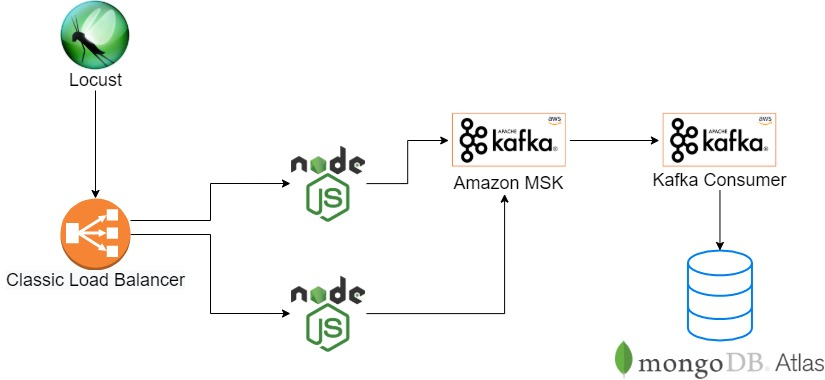
\includegraphics[width=\linewidth , height=4cm]{LaTeX/fig/system/kafka.jpeg}
    \caption{Architecture - Kafka.} 
    \end{figure}
    
    \begin{figure}[H]
    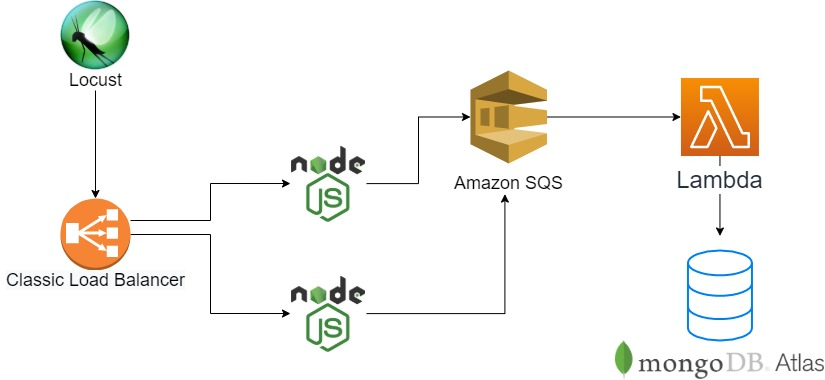
\includegraphics[width=\linewidth , height=4cm]{LaTeX/fig/system/sqs.jpeg}
    \caption{Architecture - SQS.}
    \end{figure}
\end{enumerate}
\section{Experiment Results}\label{sec:results}
\renewcommand{\labelenumi}{\alph{enumi})}
% \begin{sqsFig}
\begin{enumerate}
    \item Amazon SQS
    \begin{figure}[H]
    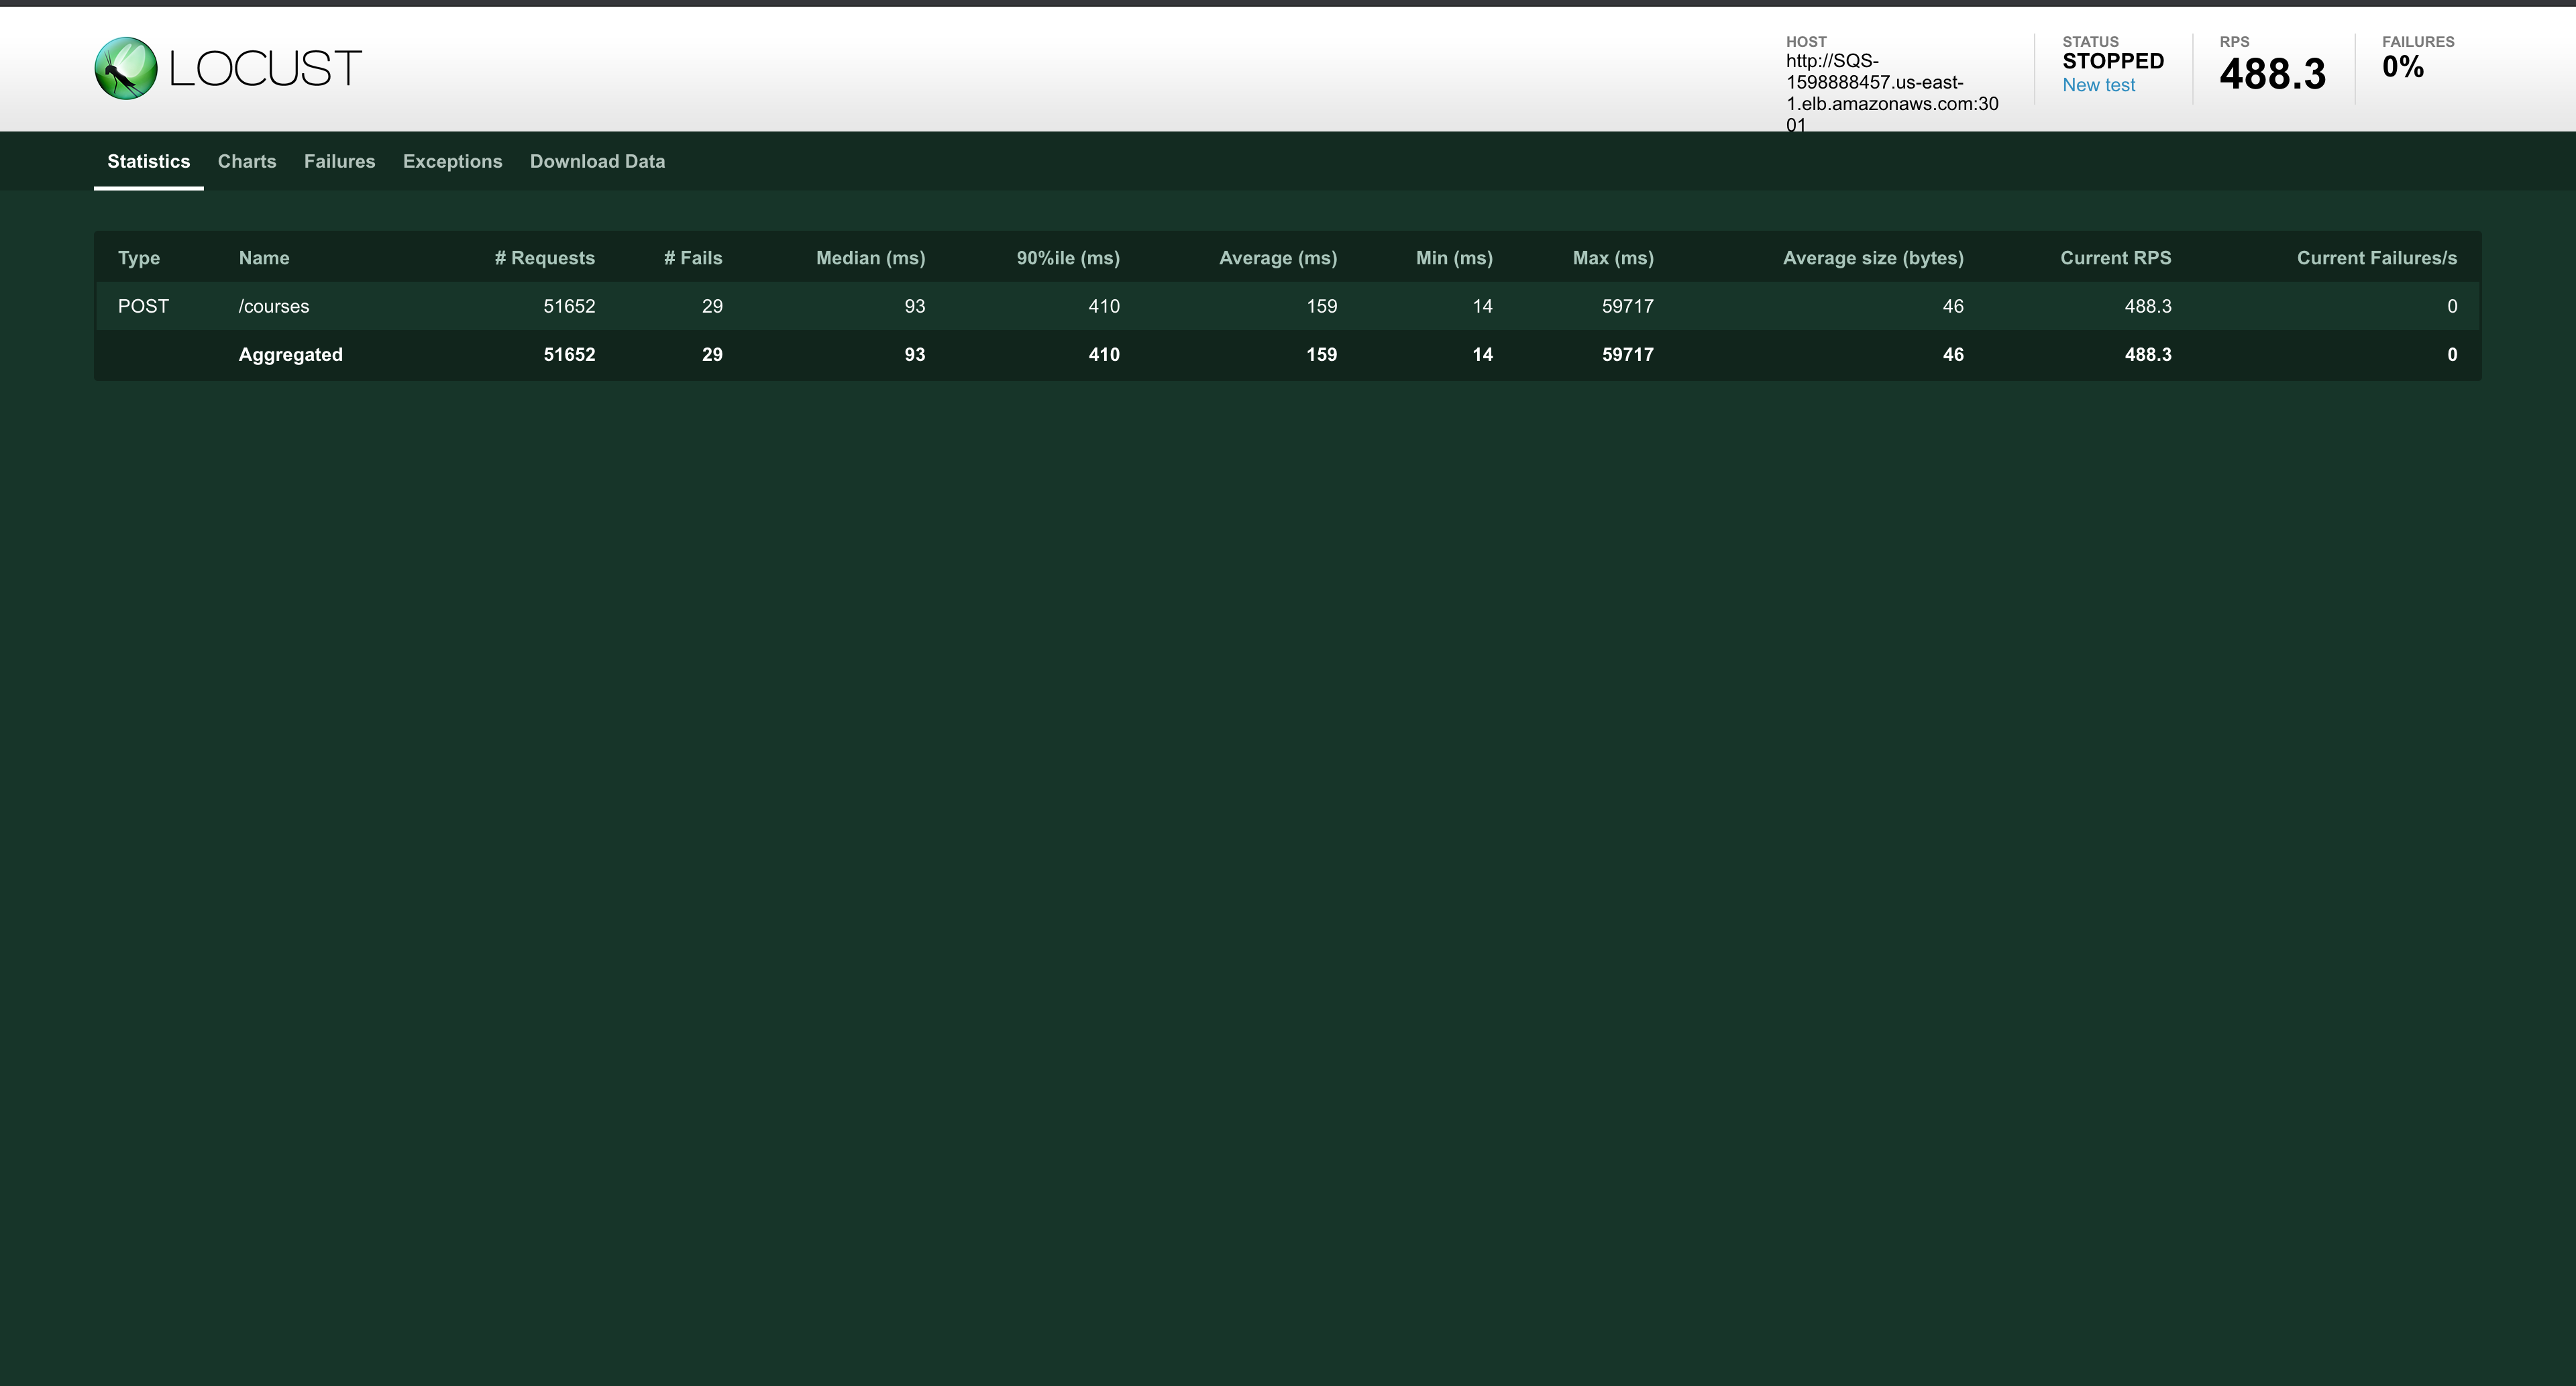
\includegraphics[width=\linewidth , height=4cm]{LaTeX/fig/sqs/locust_result.png}
    \caption{Locust result.}
    \end{figure}
    \begin{figure}[H]
    \includegraphics[width=\linewidth , height=4cm]{LaTeX/fig/sqs/number_of_users.png}
    \caption{Number of users.}
    \end{figure}
    \begin{figure}[H]
    \includegraphics[width=\linewidth , height=4cm]{LaTeX/fig/sqs/response_times_(ms).png}
    \caption{Response times.}
    \end{figure}
    \begin{figure}[H]
    \includegraphics[width=\linewidth , height=4cm]{LaTeX/fig/sqs/total_requests_per_second.png}
    \caption{Total requests per second.}
    \end{figure}
    \begin{figure}[H]
    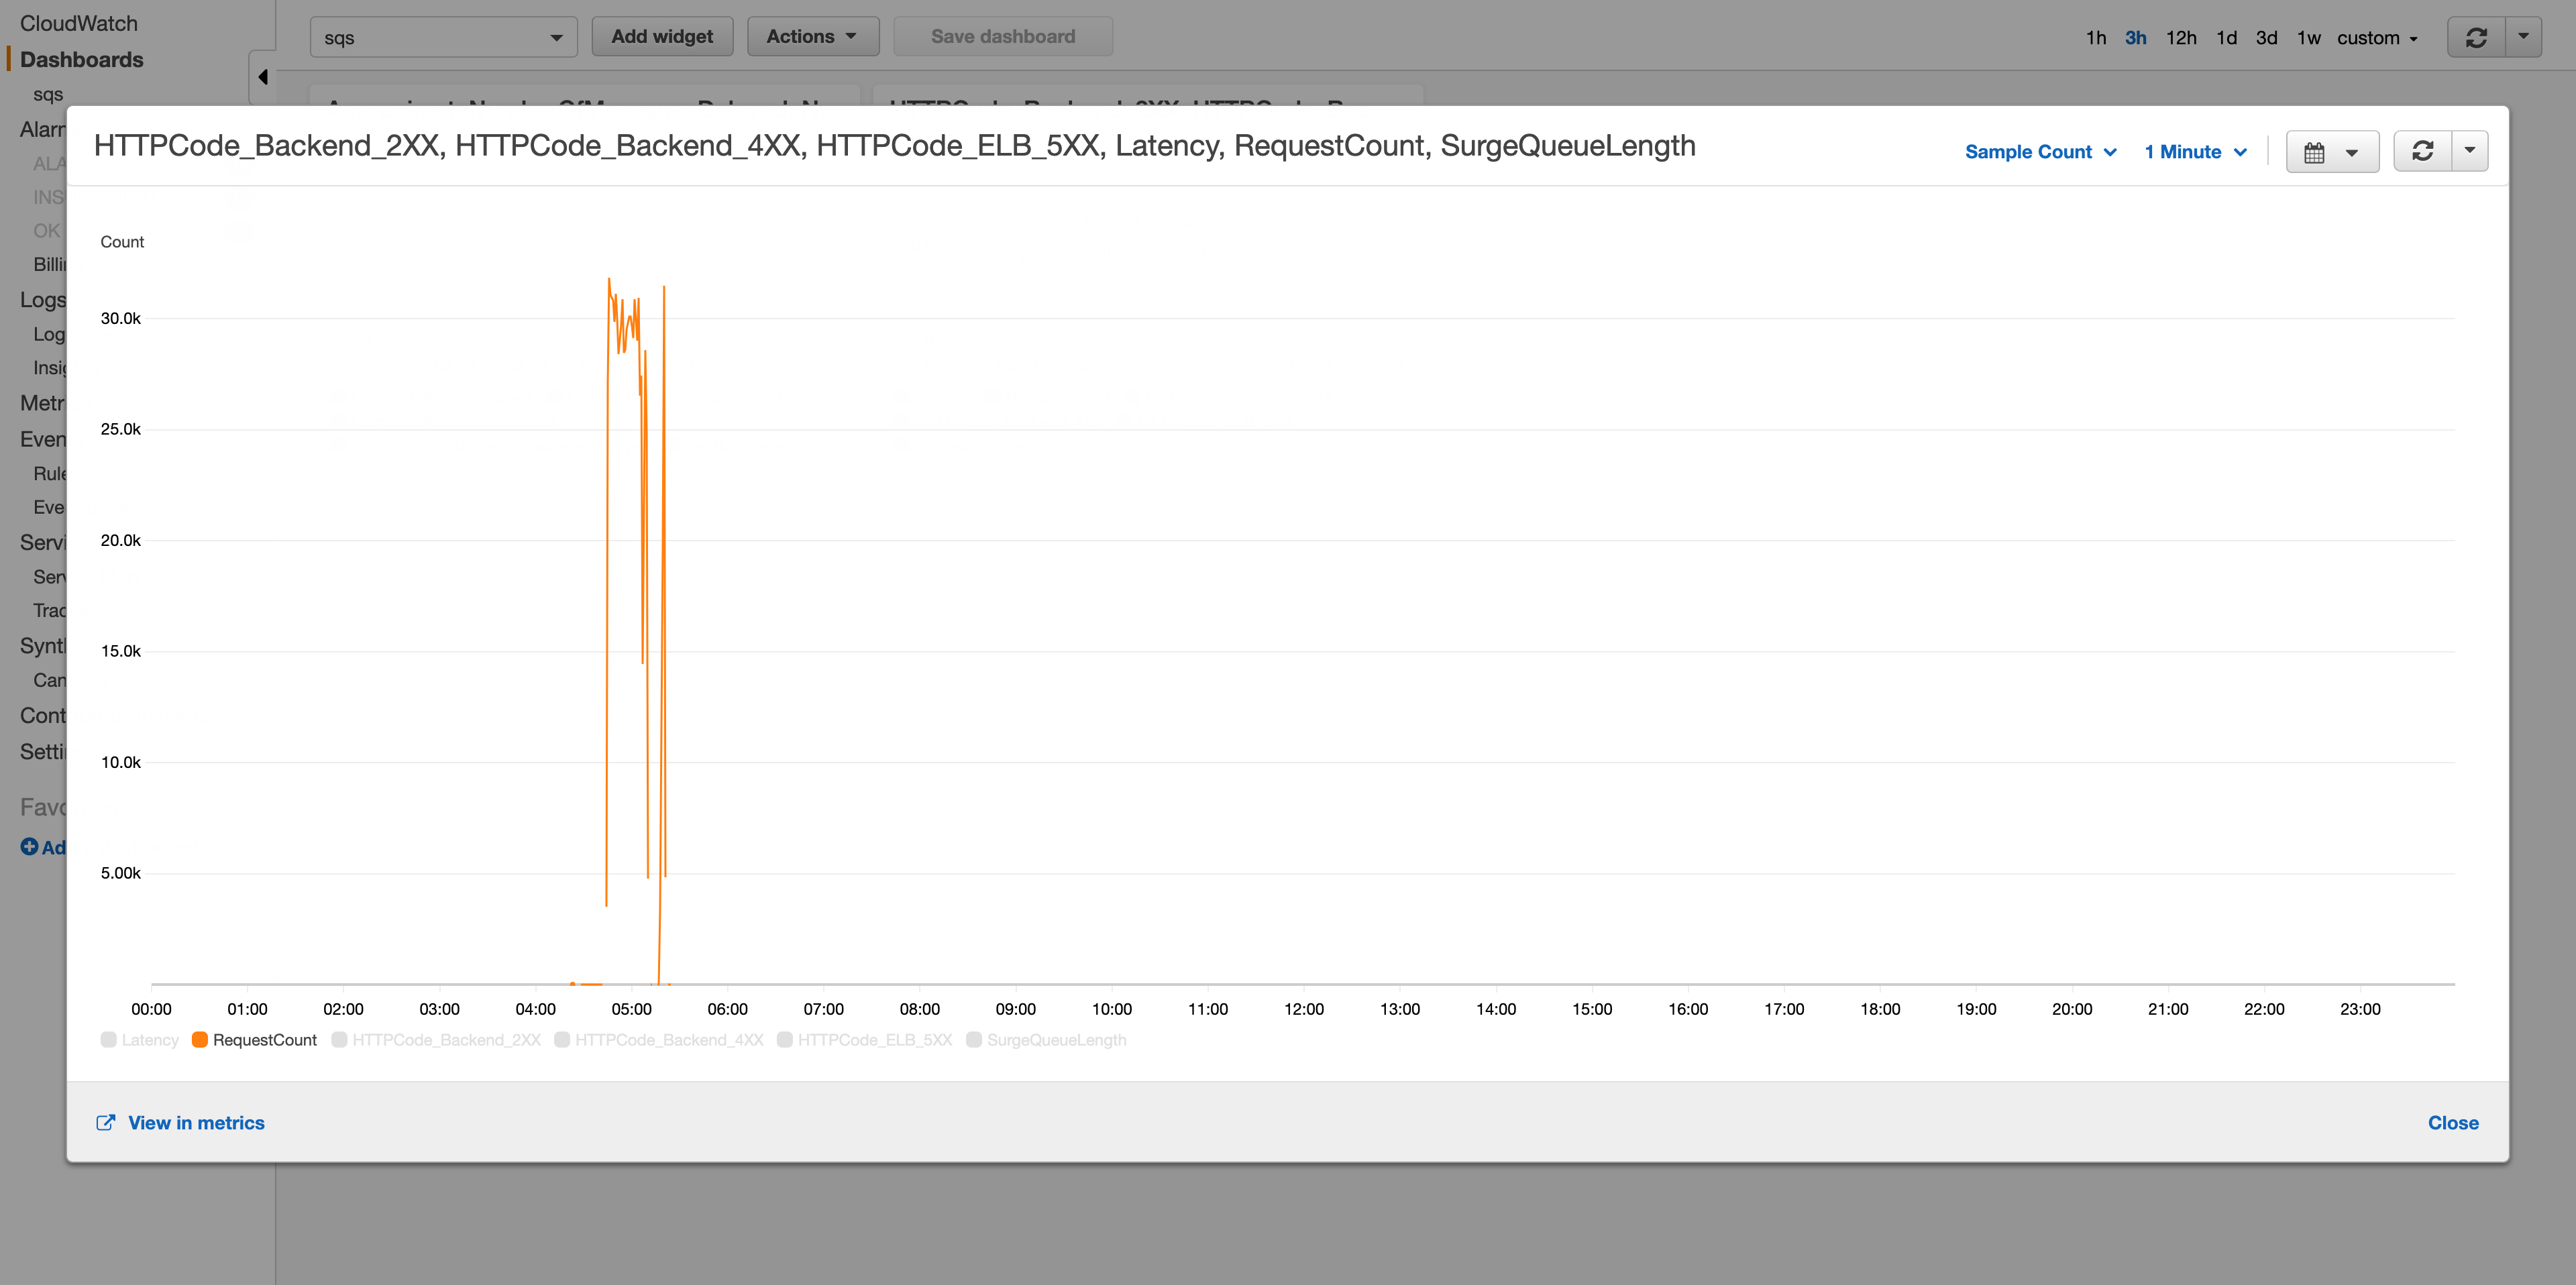
\includegraphics[width=\linewidth , height=4cm]{LaTeX/fig/sqs/request_count.png}
    \caption{Request count.}
    \end{figure}
    \begin{figure}[H]
    \includegraphics[width=\linewidth , height=4cm]{LaTeX/fig/sqs/latency.png}
    \caption{Latency.}
    \end{figure}
    \begin{figure}[H]
    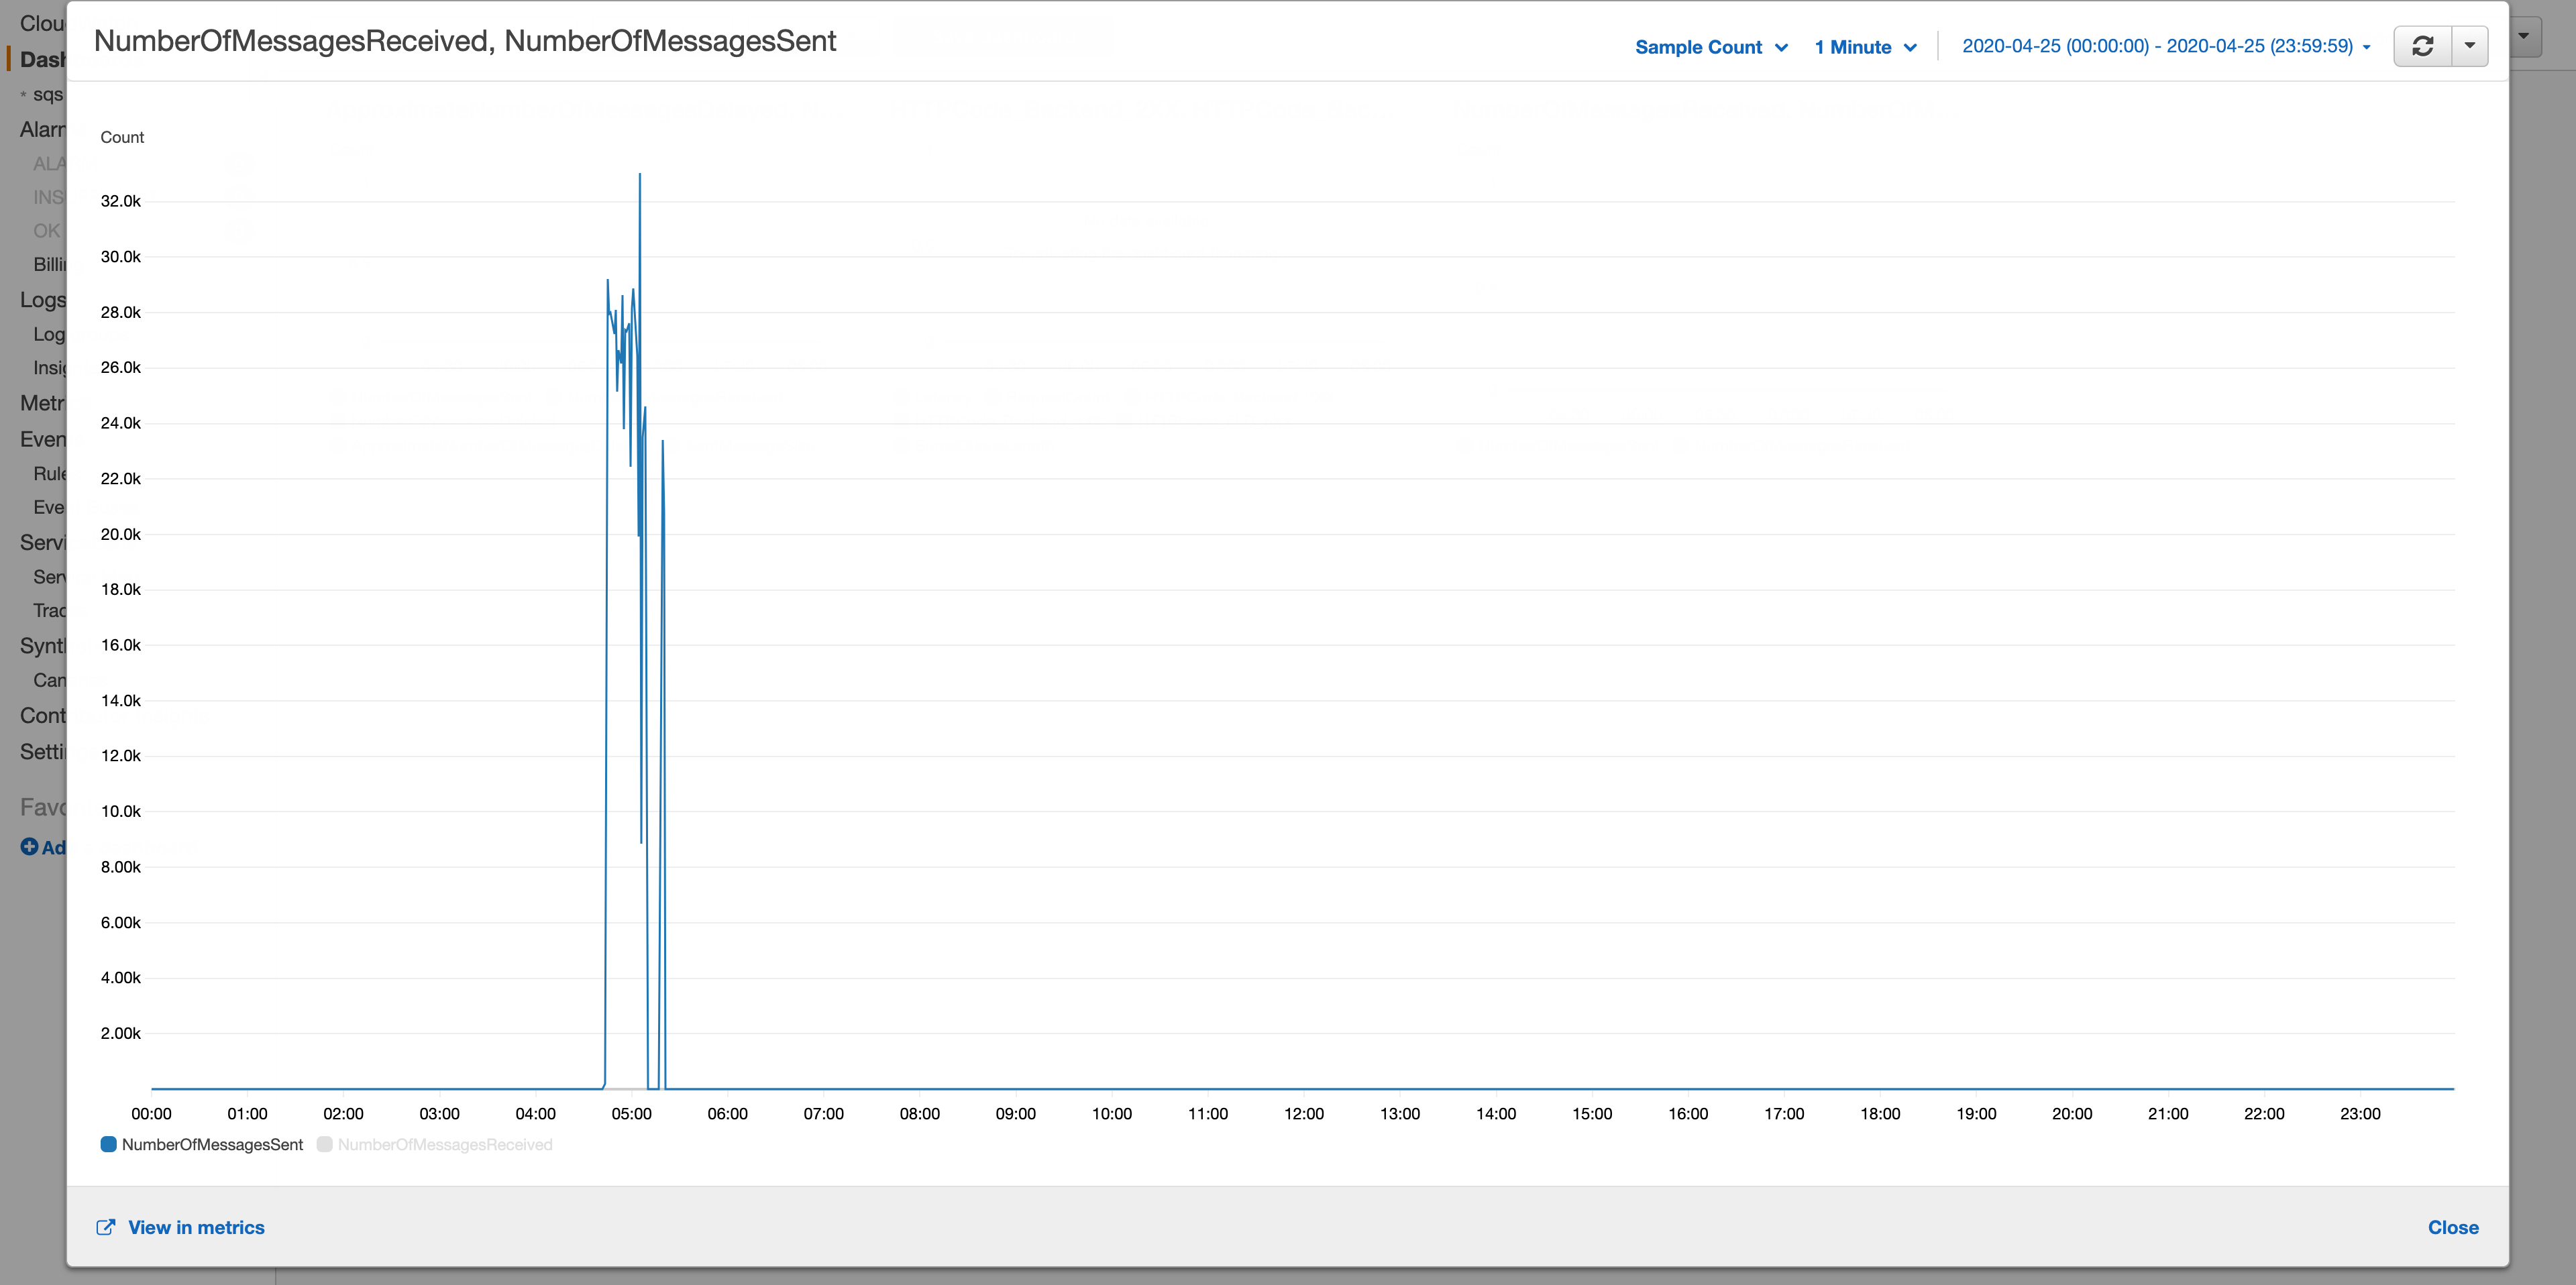
\includegraphics[width=\linewidth , height=4cm]{LaTeX/fig/sqs/msg_send.png}
    \caption{Total messages sent.}
    \end{figure}
    \begin{figure}[H]
    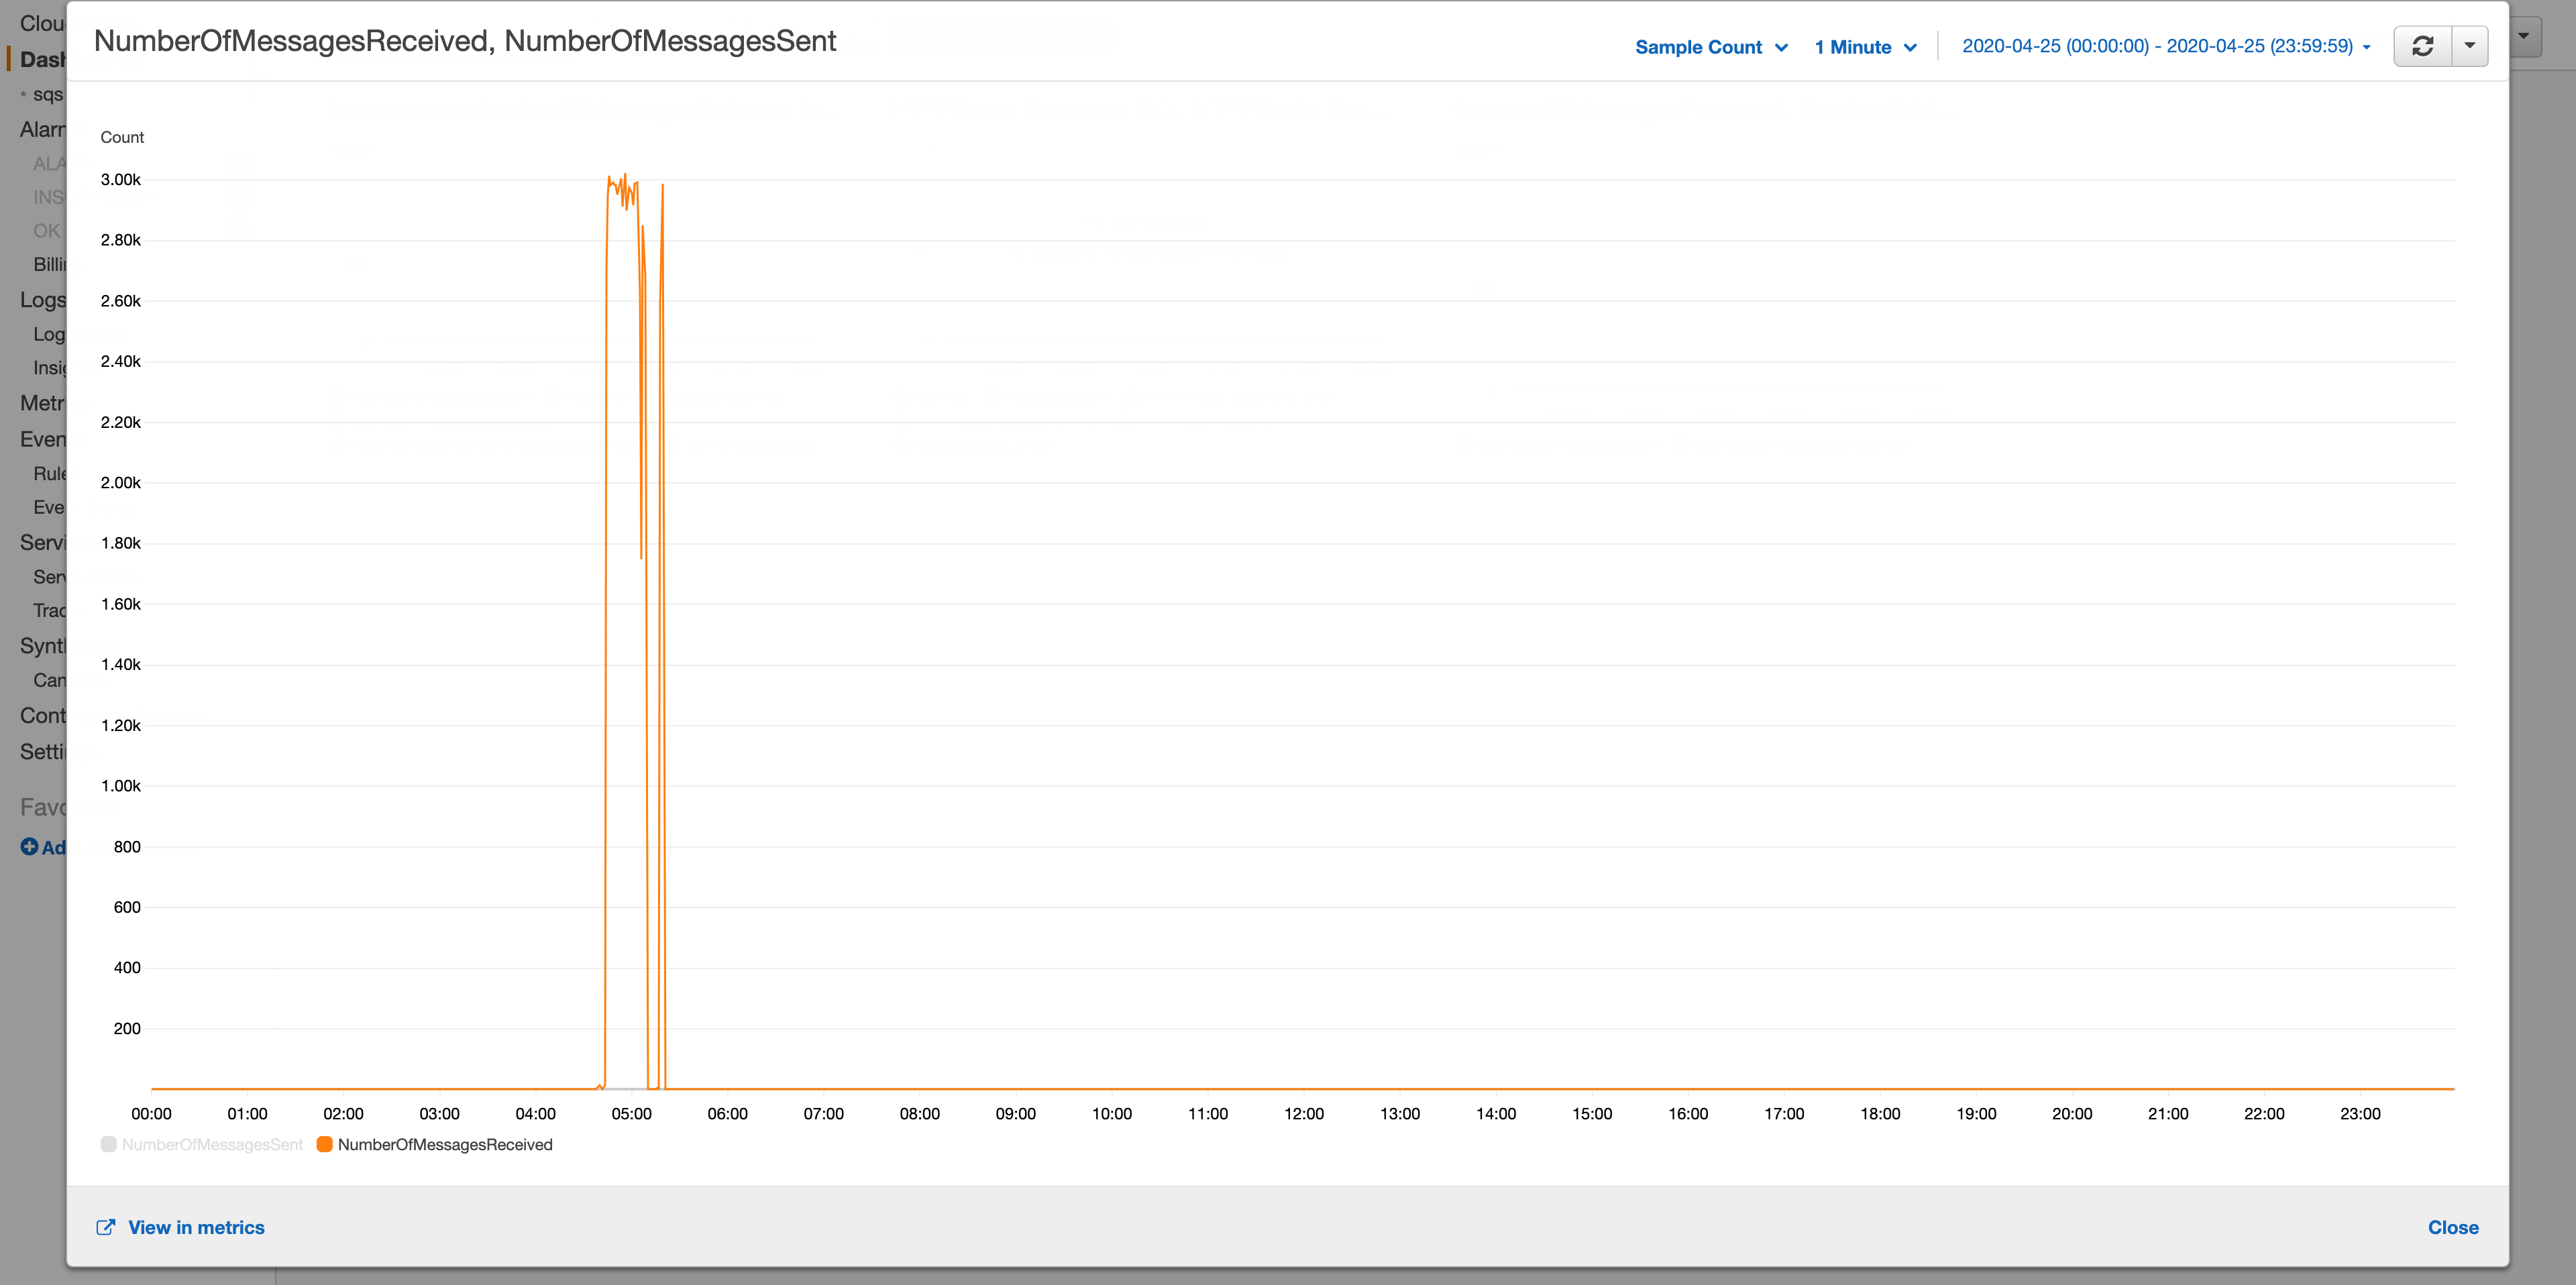
\includegraphics[width=\linewidth , height=4cm]{LaTeX/fig/sqs/msg_recieved.png}
    \caption{Total messages received.}
    \end{figure}
    
    Above shown are the results of bench marking the system using SQS. The total number of users are capped at 5000 and the hatch rate is set at 50 users/sec. \\
    \item Kafka \\
    \begin{enumerate}
        \item Non-optimized\\
        % \begin{center}
        \begin{figure}[H]
        \includegraphics[width=\linewidth , height=4cm]{LaTeX/fig/kafka/locust.png}
        \caption{Locust result.}
    \end{figure}
    \begin{figure}[H]
        \includegraphics[width=\linewidth , height=4cm]{LaTeX/fig/kafka/number_of_users.png}
        \caption{Number of users.}
    \end{figure}
    \begin{figure}[H]
        \includegraphics[width=\linewidth , height=4cm]{LaTeX/fig/kafka/response_times_(ms).png}
        \caption{Response times in ms.}
    \end{figure}
    \begin{figure}[H]
        \includegraphics[width=\linewidth , height=4cm]{LaTeX/fig/kafka/total_requests_per_second.png}
        \caption{Total requests per second.}
    \end{figure}
    \begin{figure}[H]
        \includegraphics[width=\linewidth , height=4cm]{LaTeX/fig/kafka/cpu.png}
        \caption{CPU.}
    \end{figure}
    \begin{figure}[H]
        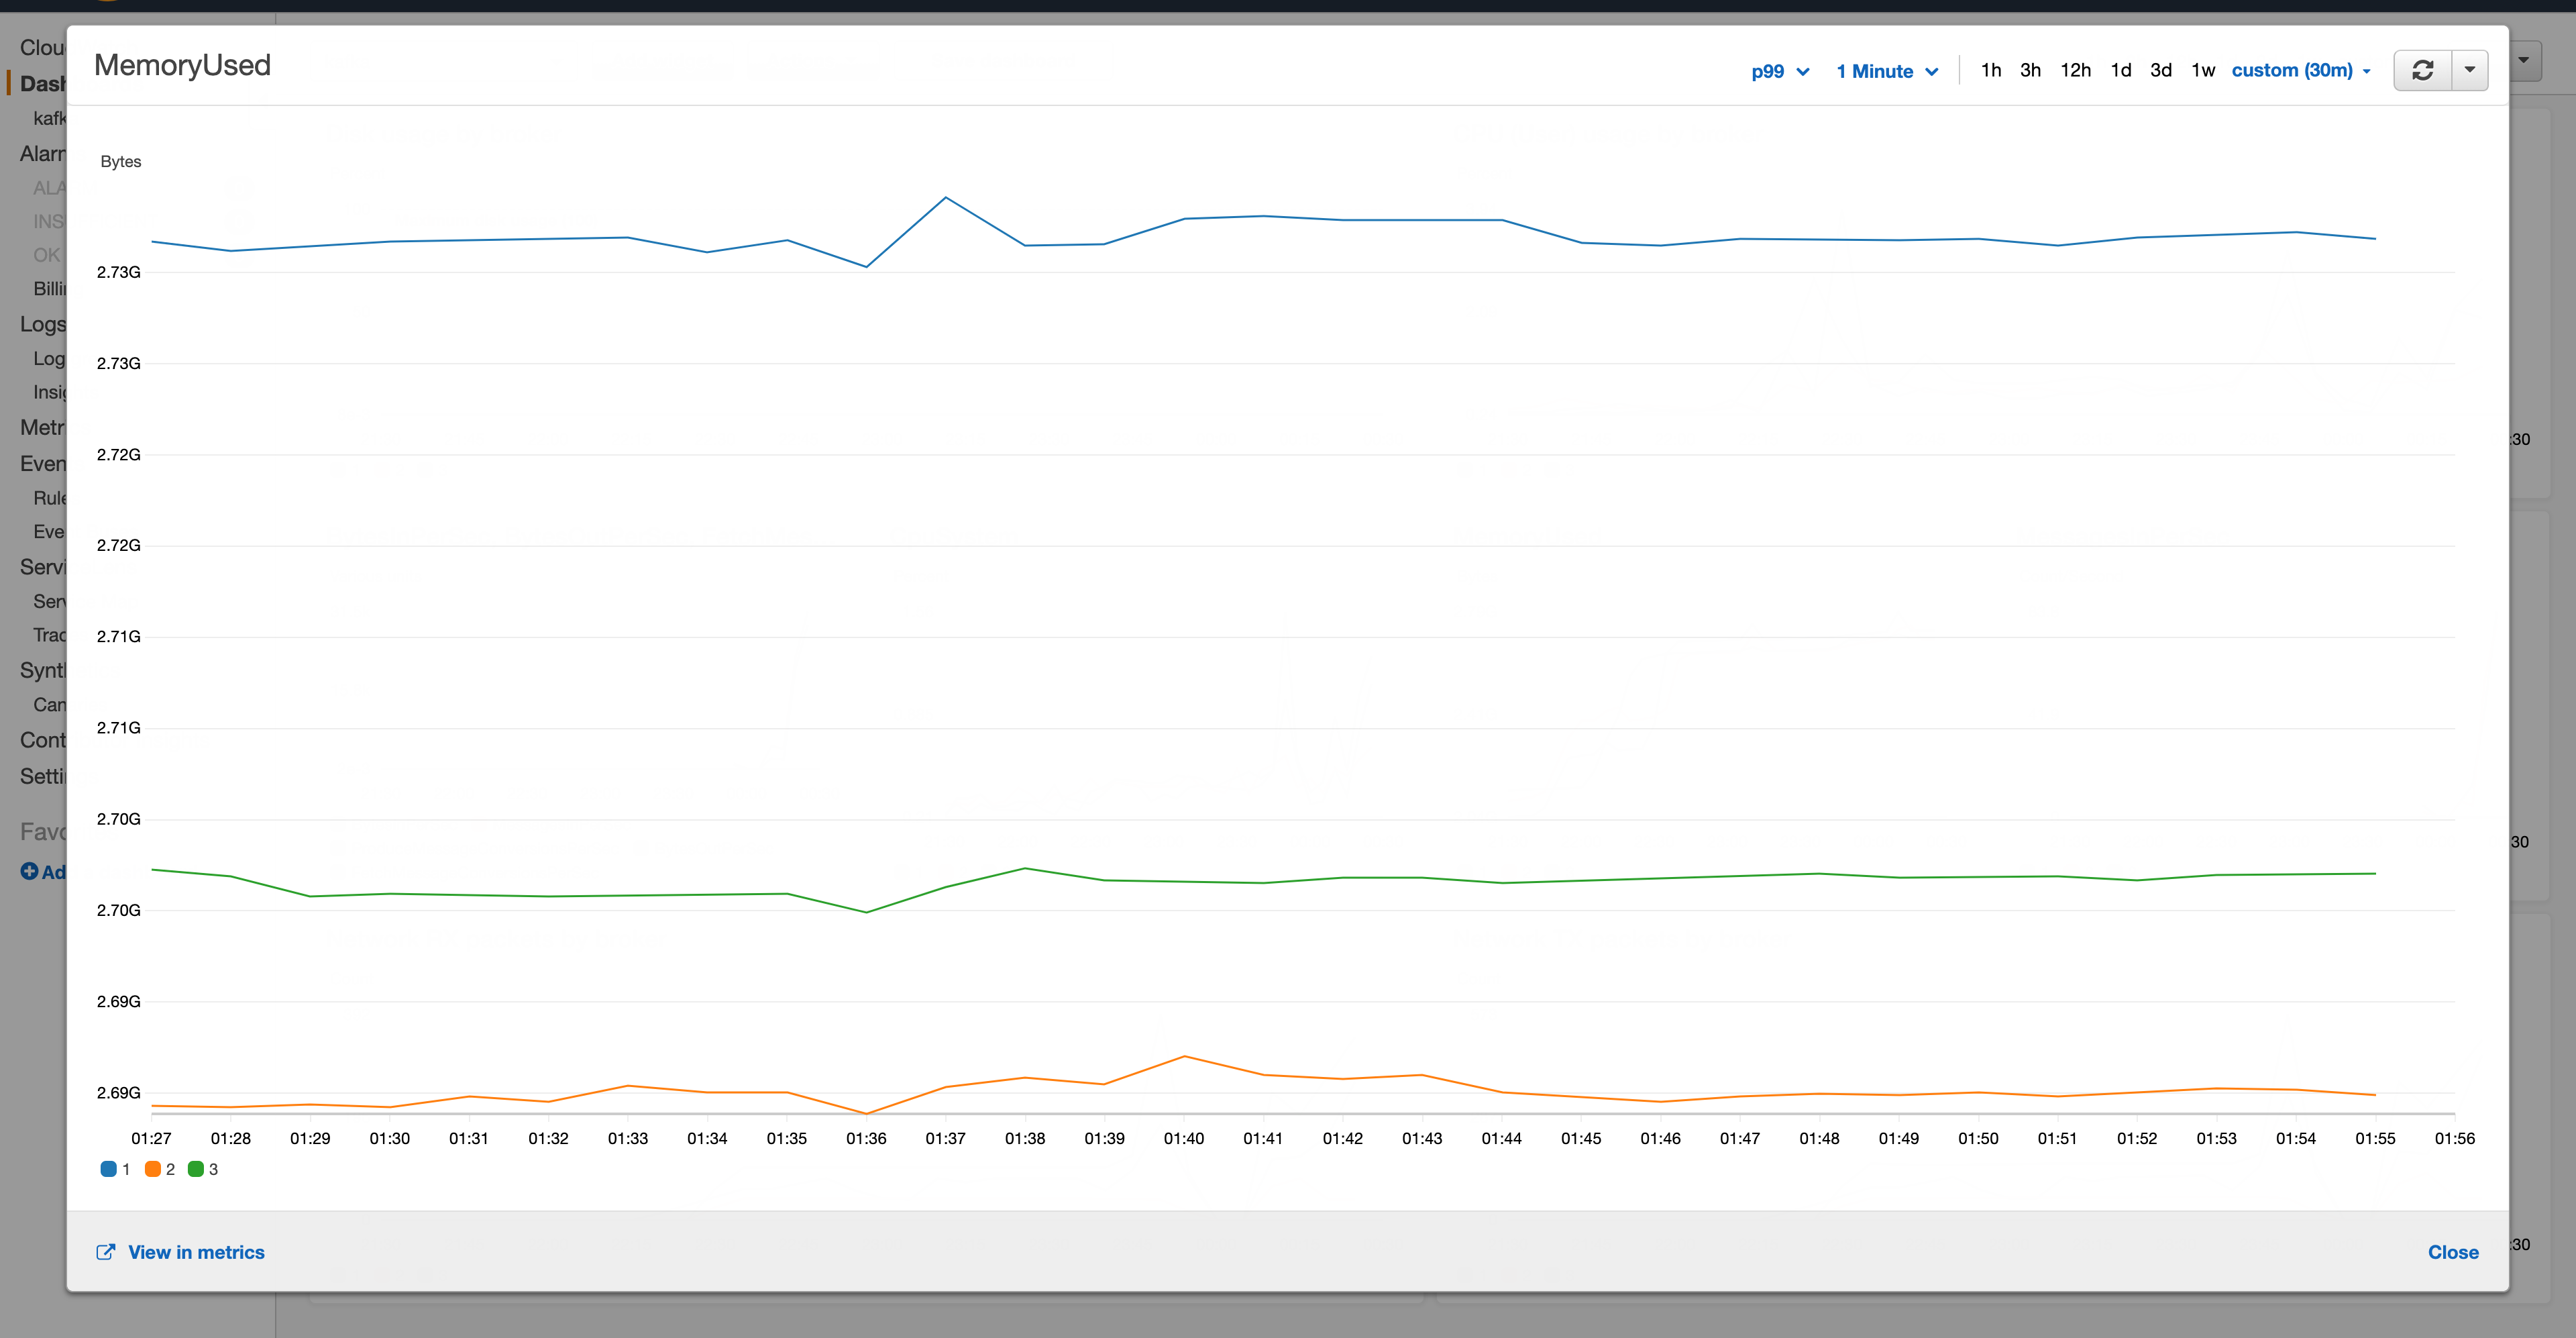
\includegraphics[width=\linewidth , height=4cm]{LaTeX/fig/kafka/memory.png}
        \caption{Memory.}
    \end{figure}
        % \end{center}
        Above shown are the results of bench marking the system using Kafka. The total number of users are capped at 5000 and the hatch rate is set at 50 users/sec. The number of brokers here are 3 and the partition size is also 3. The results on this setup are not efficient. The parallelism and the low database connection limit on the database is the problem resulting in such results.  \\\\ 
        
        
        \item Optimized \\\\
        The number of brokers are increased from 3 brokers to 6 brokers. The partition size is increased to 5 from 3. Also, the database is moved from us-west to us-east to reduce the latency. The maximum allowed connections are also increased to 1500. The following are the results of the same test on this optimized configuration.
        \begin{figure}[H]
        \includegraphics[width=\linewidth , height=4cm]{LaTeX/fig/kafka/optimized/locust.png}
        \caption{Locust result.}
    \end{figure}
    \begin{figure}[H]
        \includegraphics[width=\linewidth , height=4cm]{LaTeX/fig/kafka/optimized/number_of_users.png}
        \caption{Number of users.}
    \end{figure}
    \begin{figure}[H]
        \includegraphics[width=\linewidth , height=4cm]{LaTeX/fig/kafka/optimized/response_times_(ms).png}
        \caption{Response times in ms.}
    \end{figure}
    \begin{figure}[H]
        \includegraphics[width=\linewidth , height=4cm]{LaTeX/fig/kafka/optimized/total_requests_per_second.png}
        \caption{Total requests per second.}
    \end{figure}
    \begin{figure}[H]
        \includegraphics[width=\linewidth , height=4cm]{LaTeX/fig/kafka/optimized/cpu.png}
        \caption{CPU.}
    \end{figure}
    \begin{figure}[H]
        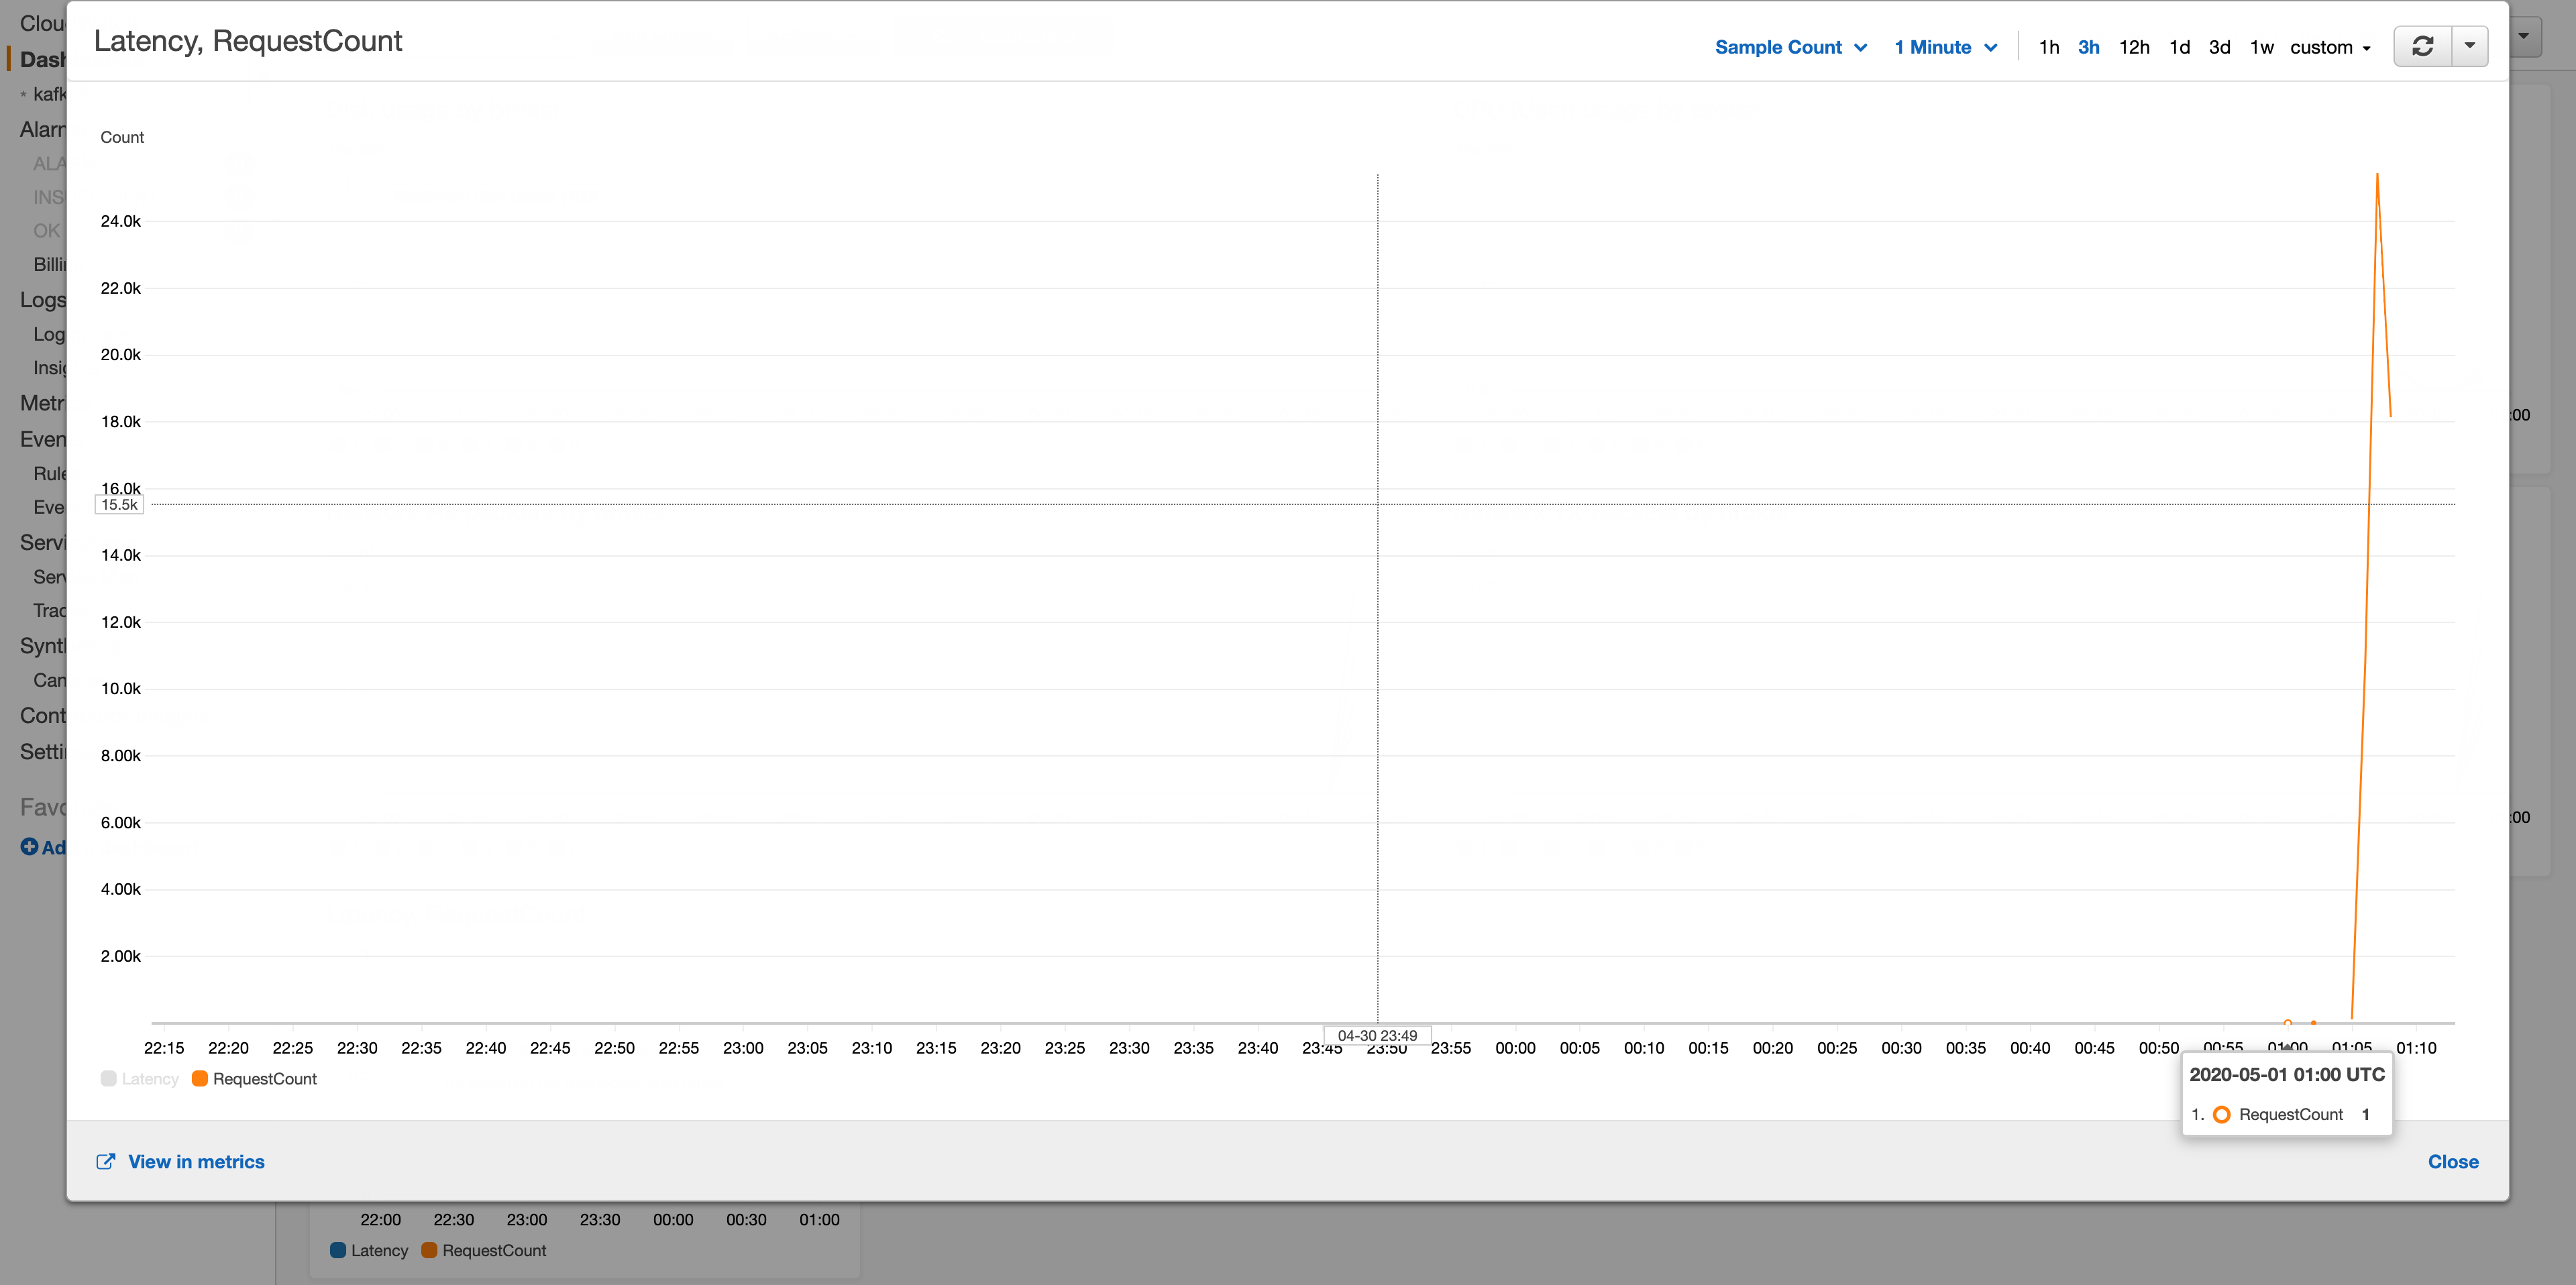
\includegraphics[width=\linewidth , height=4cm]{LaTeX/fig/kafka/optimized/req_count.png}
        \caption{Request count.}
    \end{figure}
    \begin{figure}[H]
        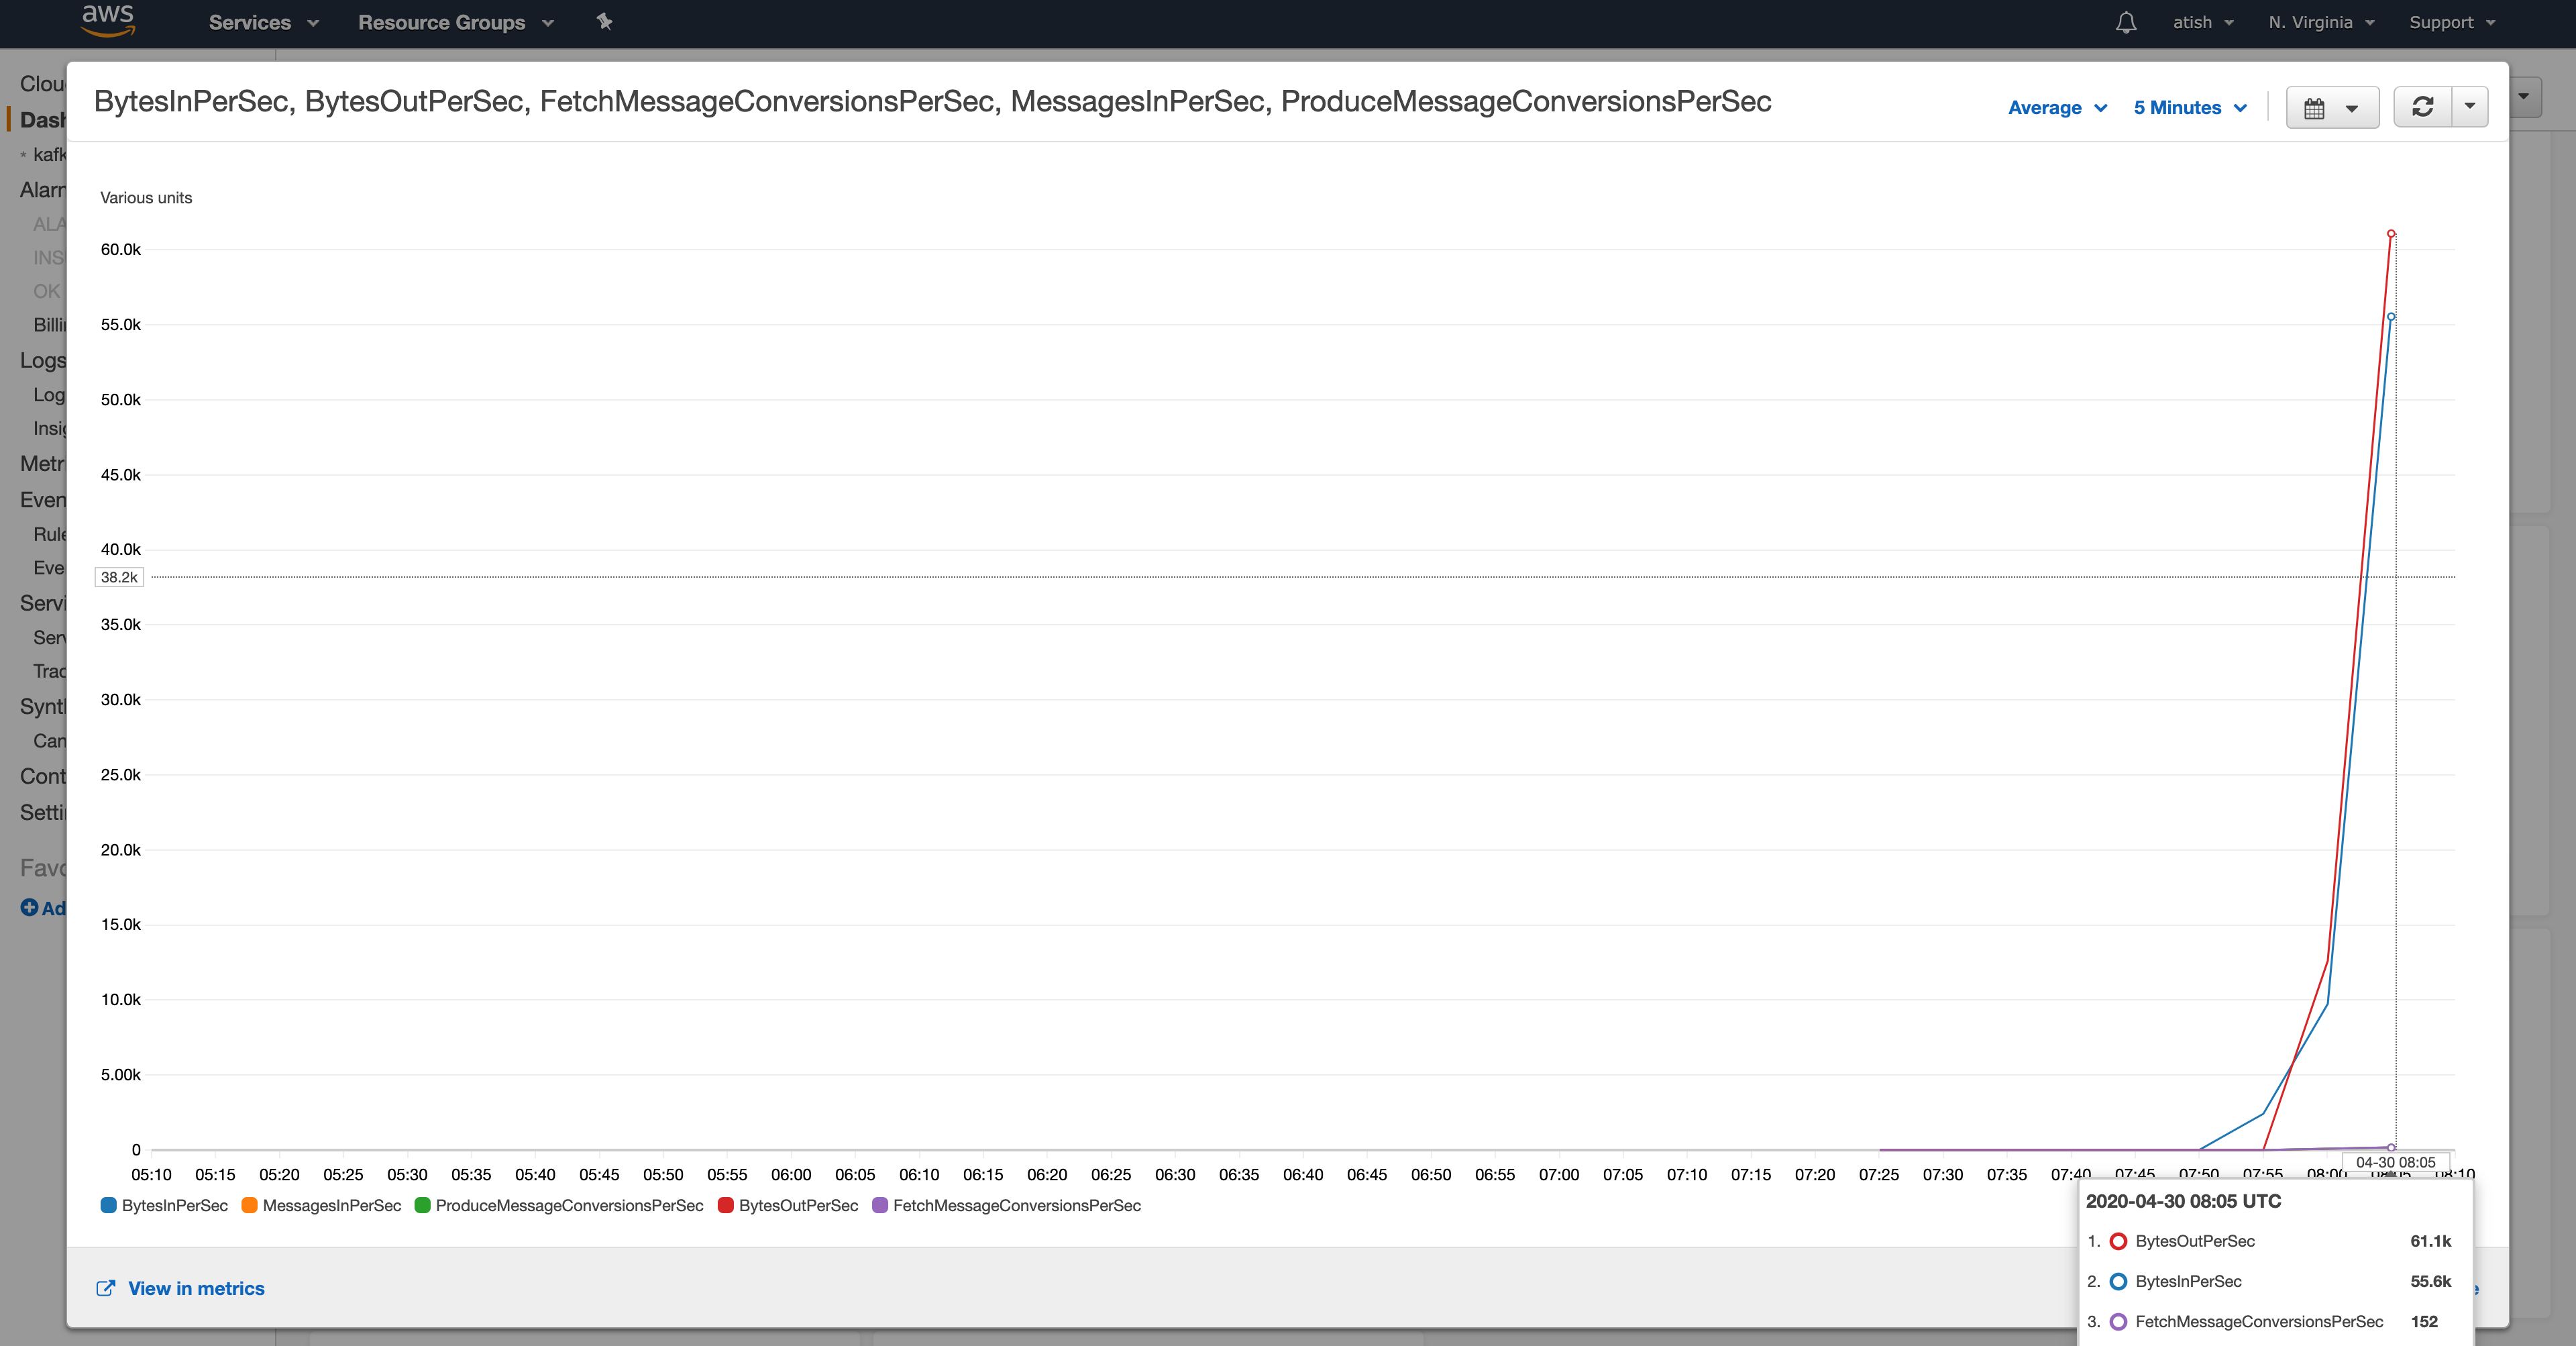
\includegraphics[width=\linewidth , height=4cm]{LaTeX/fig/kafka/optimized/bytes_in_and_out.png}
        \caption{Bytes in and out.}
    \end{figure}
    \begin{figure}[H]
        \includegraphics[width=7cm , height=4cm]{LaTeX/fig/kafka/optimized/latency.png}
        \caption{Latency.}
    \end{figure}
    \end{enumerate}
\end{enumerate}
% \end{sqsFig}
\section{Comparison}\label{sec:comparison}

\begin{enumerate}
    \item Response time:  The response time of Kafka is better than that of SQS. Also, the 90\% percentile response time of Kafka is better, which signifies that the worst performing requests of Kafka are faster than SQS.  
    \item Fails:  SQS failed on 29 requests  in our tests while Kafka failed only on 2 which suggests that Kafka is more reliable.
    \item Throughput:  The bytes-in-and-out graph shows that the bytes received and bytes sent out of Kafka increase linearly together which suggest that the throughput is high which is not the case for SQS. 
    \item Database connections:  According to our tests, we found that Kafka was heavier on database connections since the throughput is higher.
    \item Ease of implementation: SQS is categorically easier to implement and use. While Kafka needs to be monitored and configured more to get the best out of it. 
    \item Cost: SQS is priced per request. Hence if the traffic to the queues if very high the cost increases a lot. But, Kafka's pricing depend upon the instances a user uses and the storage. 
    
\end{enumerate}

\section{Conclusion}\label{sec:conclusions}
In conclusion, as seen in the results, it can be stated in this specific setup that Kafka performs better overall if response time, failure rate and throughput is taken into consideration. If the database does not support a high number of connections, SQS is the better choice. In terms of cost, if the traffic is more, Kafka is also more cost efficient as the price is not set per request.




% \bibliographystyle{IEEEtran}
% \bibliography{IEEEmybib}
\begin{thebibliography}{9}
\bibitem{KafkaVersion} 
Kafka versions,
\\\texttt{https://kafka.apache.org/22/documentation.html}

\bibitem{SQSDocumentation} 
Amazon SQS Documentation,
\\\texttt{https://docs.aws.amazon.com/AWSSimpleQueueService/}

\bibitem{MSKFaqs} 
Amazon Managed Services for Kafka FAQs,
\\\texttt{https://aws.amazon.com/msk/faqs/}

\bibitem{locust} 
Locust documentation,
\\\texttt{https://docs.locust.io/en/stable/what-is-locust.html/}

\bibitem{MDBAtlas} 
AMongoDB Atlast cluster tier,
\\\texttt{https://docs.atlas.mongodb.com/cluster-tier/}

\bibitem{AWSEC2} 
Amazon Web Services EC2 instance types,
\\\texttt{https://aws.amazon.com/ec2/instance-types/}

\end{thebibliography}

%\begin{thebibliography}{1}
%
%\bibitem{IEEEhowto:kopka}
%H.~Kopka and P.~W. Daly, \emph{A Guide to \LaTeX}, 3rd~ed.\hskip 1em plus
%  0.5em minus 0.4em\relax Harlow, England: Addison-Wesley, 1999.
%
%\end{thebibliography}

% that's all folks
\end{document}


